\documentclass{snamc2013}

%%%%%%%%%%%%%%%%%%%%%%%%%%%%%%%%%%%%%%%%%%%%%%%%%%%%%%%%%%%%%%%%%%%%%%%%%%%%%%%%
\usepackage[utf8]{inputenc} % Use UTF8 input encoding
\usepackage{graphicx}       % allows inclusion of graphics
\usepackage{booktabs}       % nice rules (thick lines) for tables
\usepackage{microtype}      % improves typography for PDF

% Configuration for source code listings
\usepackage{color}
\definecolor{gray}{rgb}{0.4,0.4,0.4}
\definecolor{darkblue}{rgb}{0.0,0.0,0.6}
\definecolor{cyan}{rgb}{0.0,0.6,0.6}
\usepackage{listings}
\lstset{
  basicstyle=\footnotesize\ttfamily,
  columns=fullflexible,
  showstringspaces=false,
  commentstyle=\color{gray}\upshape,
  frame=single
}
\lstdefinelanguage{XML}
{
  morestring=[b]",
  morestring=[s]{>}{<},
  morecomment=[s]{<?}{?>},
  morecomment=[s]{<!--}{-->},
  stringstyle=\color{black},
  identifierstyle=\color{darkblue},
  keywordstyle=\color{cyan},
  morekeywords={}
}

% Set up hyperlinking
\usepackage[breaklinks=true, linkcolor=black, citecolor=black]{hyperref}
\hypersetup{colorlinks=true, urlcolor=black,
  pdftitle={OpenMC: A State-of-the-Art Monte Carlo Code for Research and
    Development},
  pdfauthor={Paul K. Romano et al.}}

%%%%%%%%%%%%%%%%%%%%%%%%%%%%%%%%%%%%%%%%%%%%%%%%%%%%%%%%%%%%%%%%%%%%%%%%%%%%%%%%
\title{OpenMC: A State-of-the-Art Monte Carlo Code for Research and
  Development}

\author[1]{Paul K. Romano}
\author[1]{Nicholas E. Horelik}
\author[1]{Bryan R. Herman}
\author[2]{Adam G. Nelson}
\author[1]{Benoit Forget}
\author[1]{Kord Smith}

\affil[1]{Massachusetts Institute of Technology, Department of Nuclear Science
  and Engineering, 77 Massachusetts Avenue, Cambridge, MA 02139}
\affil[2]{University of Michigan, Department of Nuclear Engineering and
  Radiological Sciences, 2355 Bonisteel Boulevard, Ann Arbor, MI 48104}

\abstract{This paper gives an overview of OpenMC, an open source Monte Carlo
  particle transport code recently developed at the Massachusetts Institute of
  Technology. OpenMC uses continuous-energy cross sections and a constructive
  solid geometry representation, enabling high-fidelity modeling of nuclear
  reactors and other systems. Modern, portable input/output file formats are
  used in OpenMC: XML for input, and HDF5 for output. High performance parallel
  algorithms in OpenMC have demonstrated near-linear scaling to over 100,000
  processors on modern supercomputers. Other topics discussed in this paper
  include plotting, CMFD acceleration, variance reduction, eigenvalue
  calculations, and software development processes.}

\keywords{Monte Carlo, neutron transport, OpenMC, parallel, XML, HDF5}

\begin{document}
%%%%%%%%%%%%%%%%%%%%%%%%%%%%%%%%%%%%%%%%%%%%%%%%%%%%%%%%%%%%%%%%%%%%%%%%%%%%%%%%
\section{Introduction}

OpenMC is a relatively young Monte Carlo particle transport code, having been
developed starting in 2011 and first released to the public in December
2012. While the code does not benefit from decades of experience and feedback
from users as do other popular Monte Carlo codes such as MCNP
\cite{lanl-brown-2010} and TRIPOLI \cite{phytra-diop-2007}, it nevertheless
possesses a number of features that may be very attractive to both users and
developers.

Development of OpenMC was spearheaded by the Computational Reactor Physics Group
(CRPG) at Massachusetts Institute of Technology (MIT) as part of a project to
develop scalable parallel algorithms for future exascale supercomputers. While
this was the original focus of the code development efforts, there are now a
wide variety of research and development efforts underway using OpenMC. In the
last year, the development team has also grown to span multiple
organizations.

Various aspects of the OpenMC code have been described previously
\cite{ane-romano-2013, mc-romano-2013}. However, due to the developmental nature
of the code, many changes have been, and continue to be, made. The objective of
the present work is to give a fairly complete and up-to-date overview of the
present capabilities and features of OpenMC.

%%%%%%%%%%%%%%%%%%%%%%%%%%%%%%%%%%%%%%%%%%%%%%%%%%%%%%%%%%%%%%%%%%%%%%%%%%%%%%%%
\section{Methods}

\subsection{Physics}

At the present time, OpenMC is capable of simulating only neutrons either in
fixed source\footnote{Subcritical multiplication problems are not yet
  supported.} or $k$-eigenvalue problems. The data governing the interaction of
neutrons with various nuclei are represented using the ACE format
\cite{lanl-x5-2008-ace} which is also used by MCNP and Serpent
\cite{vtt-leppanen-2012}. ACE-format data can be generated with the NJOY nuclear
data processing system \cite{lanl-macfarlane-1994} which converts raw ENDF/B
data into a representation that is suitable for use in a Monte Carlo code. The
use of a standard cross section format allows for a direct comparison of OpenMC
with other codes since the same cross section libraries can be used. However,
the downside is that the implementation of physical methods is necessarily
limited by the data that is available in the ACE format.

An indexing technique \cite{ane-leppanen-2009} based on pointers is used to
speed up energy grid searches when calculating cross sections. For problems with
tens of nuclides or less, the indexing technique provides a considerable
performance benefit with modest additional memory requirements. However, with
hundreds of nuclides in a problem, the memory requirements may become too
prohibitive. As a result, alternative energy grid treatments are now being
explored.

OpenMC is capable of faithfully simulating all nuclear reactions producing
secondary neutrons, including $(n,2n)$, $(n,3n)$, fission, and level inelastic
scattering, according to the various secondary energy and angle distribution
laws in the ACE format data. Photon transport capability has not yet been
implemented, and thus OpenMC does not explicitly track photon production
resulting from $(n,\gamma)$ or fission reactions.

To properly treat scattering kinematics when the target nucleus is not at rest,
OpenMC uses a free gas approximation \cite{mc-sutton-2009} wherein the
velocities of the target nuclei are sampled from a Maxwellian distribution. For
thermal neutrons scattering from bound molecules such as hydrogen or deuterium
in water, graphite, beryllium, etc., the free gas approximation will not
accurately capture the scattering kinematics and $S(\alpha,\beta,T)$ scattering
law data must be used. The $S(\alpha,\beta,T)$ data are given on ACE files
separate from the normal nuclide data. To account for self-shielding in the
unresolved resonance range, OpenMC uses the probability table method
\cite{nse-levitt-1972}. Probability tables are included in the ACE data for many
nuclides.

The method of successive generations \cite{nukleonik-lieberoth-1968} is used to
solve $k$-eigenvalue problems. The user also has the option to group multiple
generations into a ``batch'' to reduce correlation between realizations of the
tally random variables \cite{physor-kelly-2012}. Like MCNP, OpenMC keeps track
of the collision, absorption, and track-length estimators of $k_{eff}$ and then
calculates a minimum-variance combined estimator based on the covariance matrix
of the three single estimators. To assess convergence of the source
distribution, the user can also define a mesh over which the Shannon entropy
should be calculated.

\subsection{Geometry}

In order to model arbitrarily complex geometric objects, OpenMC uses a
constructive solid geometry representation. In the current implementation,
closed volumes, or \textit{cells}, can be represented as the intersection of
multiple \textit{half-spaces}. Each half-space is in turn defined as the
positive or negative side of a plane or quadratic surface. This allows curved
surfaces such as spheres and cylinders to be modeled exactly with no error due
to mesh discretization. Most geometries of interest in particle transport can be
modeled with first and second-order surfaces with the exception of some exotic
geometries, e.g., a torus in a fusion system where a fourth-order equation is
required. The restriction of closed volumes to only those that are formed by the
intersection of surfaces (so-called simple cells) results in greater simplicity
of the geometry implementation. However, the burden is shifted to the user who
may then need to break up certain closed volumes into multiple cells.

In addition to the simple geometry constructs described above, OpenMC provides
constructs that allow the user to model a two or three-dimensional structured
mesh consisting of quadrilaterals. These constructs are useful for modeling the
core and assembly layout in a variety of commercial and research reactor
designs. As in MCNP and Serpent, these repeated structures are handled through
the use of \textit{universes}, a collection of cells occupying all of space that
may be substituted within another closed volume. A universe may also be
translated and/or rotated. Transmitting, vacuum, or reflective boundary
conditions can be applied to any surface, thus giving the user full flexibility
in the treatment of boundaries.

\subsubsection{Geometry Plotting}

Currently two different plotting capabilities are available in OpenMC. The first
is a 2D raster plotting capability that allows the user to visualize the
geometry along a cut plane. Plots can be colored by unique material or cell, and
users have the option to selectively include/exclude certain regions. The 2D
plot is written to a portable pixmap (.ppm) file which is natively viewable on
many Linux distributions. Since the PPM file is uncompressed, an image
converting utility can significantly reduce the size of the plot by converting
it to a compressed format such as portable network graphics
(.png). \autoref{fig:atr} shows a 2D raster plot of a model of the Advanced Test
Reactor (ATR).
\begin{figure}[htb]
  \centering
  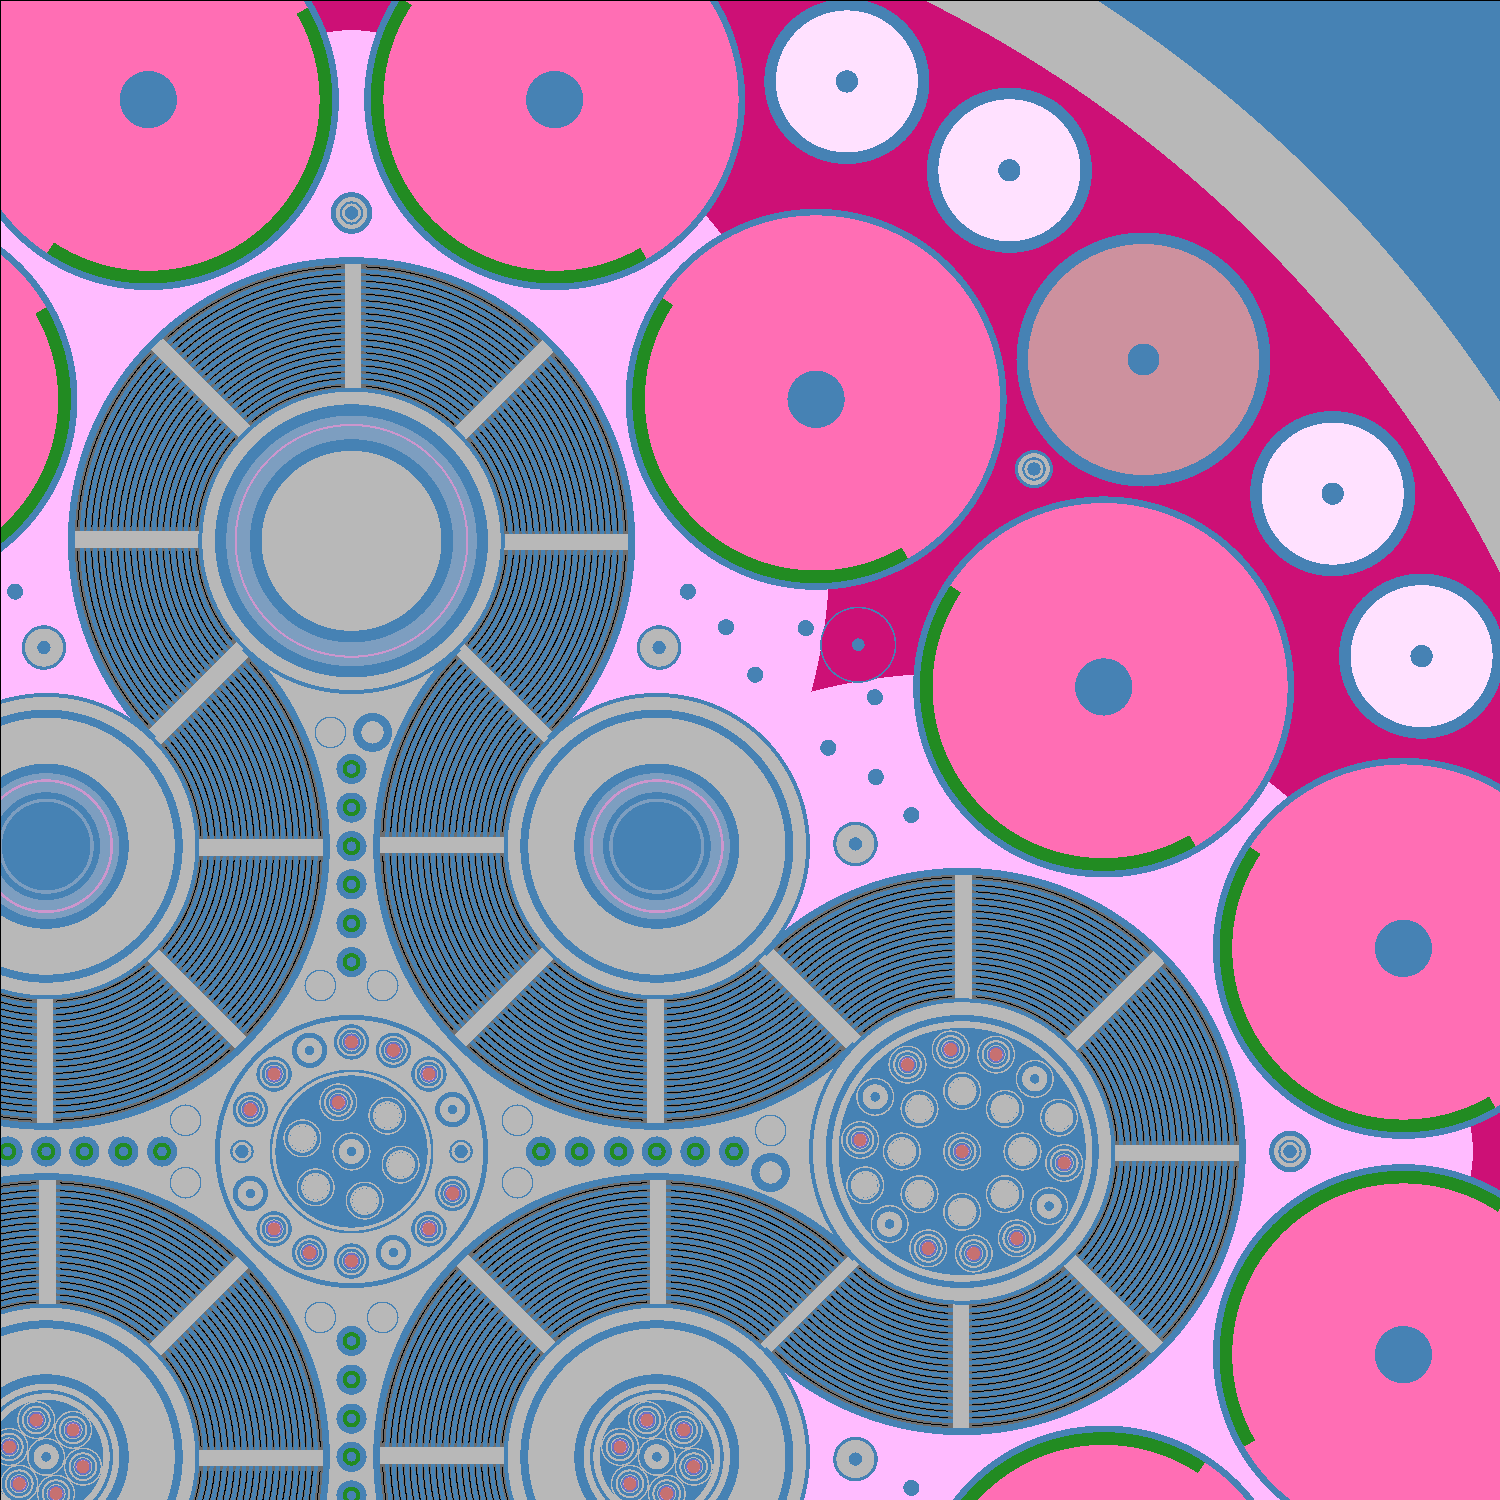
\includegraphics[width=0.4\textwidth]{images/atr.png}
  \caption{Cross-sectional view of a section of an OpenMC model of the Advanced
    Test Reactor (ATR).}
  \label{fig:atr}
\end{figure}

In addition to 2D raster plotting, a new plotting capability has been added to
OpenMC that allows for the visualization of geometry in 3D using standard
viewers such as ParaView and Visit. By specifying a uniform rectilinear grid of
voxels (analogous to image pixels), users can produce a binary file containing
the cell or material ids for each cell in the grid.  These files are created
with the same raster method used by the 2D plotter in OpenMC, where a
'find\_cell' routine is called to determine the attributes of the geometry at
each voxel center.  Since this 'find\_cell' routine is the same one used during
simulation, the voxel information produced by this method is representative of
the actual simulation geometry, limited only by the user-specified granularity
of the voxels.

Once the voxel binary file is produced, users can process the data into a
standard 3D datafile and visualize however desired.  For convenience, a Python
utility is provided to convert voxel files into either SILO or VTK files that
can be viewed in many well-established 3D data visualization tools. The example
provided by this utility easily enables users to write custom scripts that
section geometry features or mask specific cells or materials. For example,
\autoref{fig:grid-spacer} and \autoref{fig:burnable-absorber} show plots of a
PWR grid spacer and burnable absorber pin, respectively, with various materials
and features clipped for easy inspection of the geometry.
\begin{figure}[htb]
  \centering
  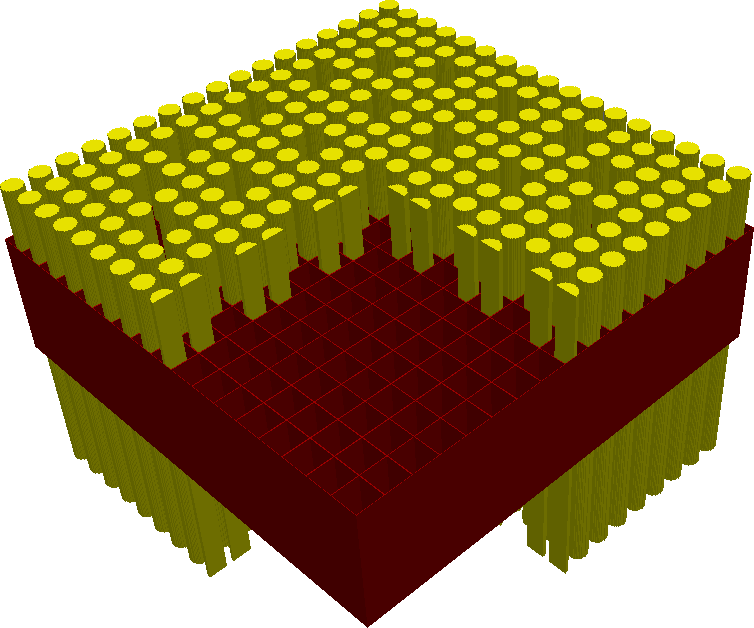
\includegraphics[width=0.4\textwidth]{images/spacer.png}
  \caption{3D plot of a grid spacer in the BEAVRS benchmark
    \cite{mc-horelik-2013} as shown in ParaView.}
  \label{fig:grid-spacer}
\end{figure}
\begin{figure}[htb]
  \centering
  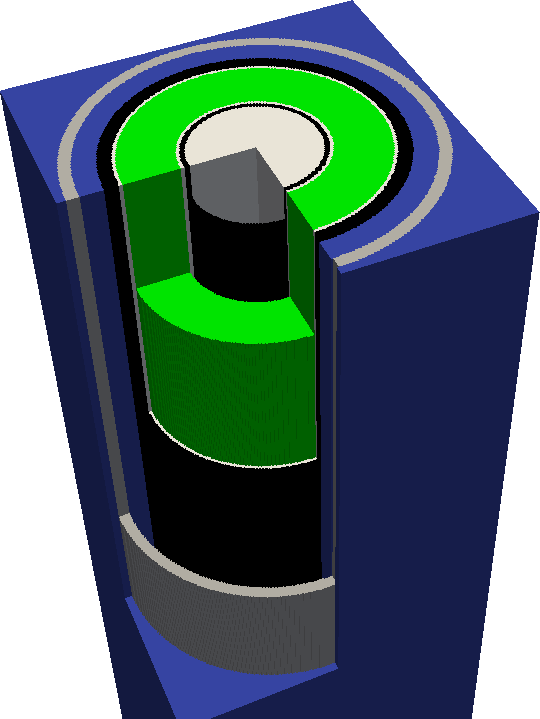
\includegraphics[width=0.3\textwidth]{images/ba.png}
  \caption{3D plot of a burnable absorber pin in the BEAVRS benchmark as shown
    in ParaView.}
  \label{fig:burnable-absorber}
\end{figure}

\subsection{Tallies}

OpenMC has a flexible, low-overhead tally system which enables users to obtain
physical results of interest. Tallies are defined by combinations of
\textit{filters} and \textit{scores}, borrowing terminology from a paper by
Sutton et al. \cite{mc-sutton-2007}. Each filter limits what events can score to
the tally based on the attributes of the particle. For example, a filter could
limit scoring events to particles traveling within a specified cell or a
specified range of pre-collision energies. A full and up-to-date list of filters
which may be applied to tallies can be found in the OpenMC User's Guide
\cite{romano-2013-doc}. Each score identifies an actual physical quantity to be
scored upon an event which matches the specified filters. Some examples of valid
scores include the flux, fission reaction rate, neutron production rate, or
local energy deposition from fission. In addition to a set of defined scores, it
is also possible to obtain reaction rates for an arbitrary MT value. Users also
have the option of scoring tallies for specific nuclides within a material. If
no nuclides are specified, macroscopic cross sections for the material are used
in determining scores.

With filters for pre- and post-collision energy and scoring functions for
scattering and fission production, it is possible to use OpenMC to generate
cross sections with user-defined group structures. The coarse mesh finite
difference (CMFD) solver within OpenMC, discussed at length later, uses the
tally system directly to obtain multi-group cross sections.

All tallies are scored using a track-length estimator by default. However, for
tallies requiring post-collision attributes of the particle, e.g., scattering
moments, a collision estimator is used instead. Users can also explicitly
specify that the track-length or collision estimator should be used for a given
tally.

Historically, some Monte Carlo codes have suffered severe performance penalties
when tallying a large number of quantities \cite{pnst-vanveen-2011}. Care must
be taken to ensure that a tally system scales well with the total number of
tally bins. In OpenMC, a mapping technique is used that allows for a fast
determination of what tally/bin combinations need to be scored to a given
particle's phase space coordinates. For each discrete filter variable, a list is
stored that contains the tally/bin combinations that could be scored to for each
value of the filter variable. If a particle is in cell $n$, the mapping would
identify what tally/bin combinations specify cell $n$ for the cell filter
variable. In this manner, it is not necessary to check the phase space variables
against each tally. Note that this technique only applies to discrete filter
variables and cannot be applied to energy bins. For energy filters, it is
necessary to perform a binary search on the specified grid.

\subsection{Parallelism}

OpenMC is capable of running in parallel using the message passing interface
(MPI). Particles within a batch are divided equally among processes such that
each processor has approximately the same amount of work to perform. Results of
a parallel calculation are reproducible, i.e. the same result is given
regardless of the number of processors that is used. At the time of writing, an
implementation of shared-memory parallelism via the OpenMP API is still under
development.

A substantial amount of research and development related to OpenMC has focused
on scalable parallel algorithms. This R\&D has culminated in the development of
two algorithms which have enabled nearly linear scaling to over 100,000
processes. The first algorithm is related to the collection and sampling of
fission sites, which are stored in an array known as the \textit{fission
  bank}. The algorithm forgoes a typical master-slave communication pattern in
favor of nearest-neighbor exchanges of fission/source sites. A derivation and
analysis of the algorithm complexity is given in Romano and
Forget\cite{nse-romano-2012}; the salient point is that nearest-neighbor
exchanges, in the context of this algorithm, have an expected communication cost
$O(\sqrt{N/p})$ whereas the computational work scales as $O(N/p)$. Thus,
arbitrarily good scaling can be achieved. Previous scaling results were reported
in~~\cite{ane-romano-2013} for the Jaguar supercomputer at Oak Ridge National
Laboratory. Those results alongside with new scaling results on the Intrepid
Blue Gene/P supercomputer at Argonne National Laboratory are shown in
\autoref{fig:scaling}.
\begin{figure}[htb]
  \centering
  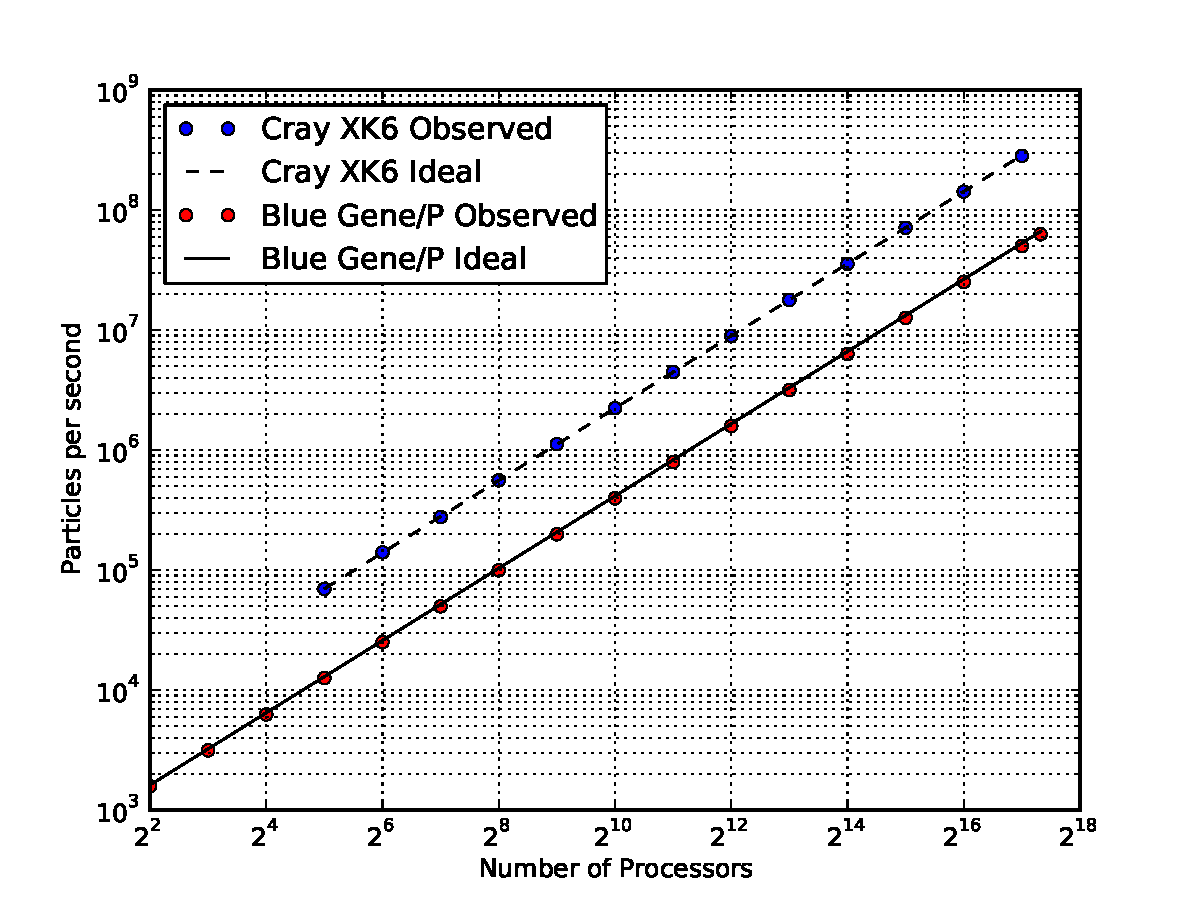
\includegraphics[width=0.5\textwidth]{images/scaling_loglog.pdf}
  \caption{Parallel scaling for the Monte Carlo Performance Benchmark on the
    Cray XK6 (Jaguar) and Blue Gene/P (Intrepid) supercomputers.}
  \label{fig:scaling}
\end{figure}

While the novel fission bank algorithm substantially reduces communication
between fission generations, it is still necessary to combine tally results from
multiple processors which might entail significant network communication. The
communication associated with synchronizing tallies across processors is
proportional to both the number of processors and the number of tally
bins. Thus, for problems with very large tally requirements, and hence large
computational requirements, this source of communication can erode parallel
efficiency. It was shown in \cite{trans-romano-2012} that by grouping
realizations of tally random variables over successive generations rather than
over multiple processors, the communication associated with tallies can be
reduced dramatically. While the reported sample means will not change when this
technique is employed, the variance of the sample mean will in general be
different. However, the expected value of the variance remains the same. A user
input option is available in OpenMC that modifies the grouping of tally results
to reduce overall communication.

\subsection{Variance Reduction}

Extensive variance reduction techniques are not yet available in
OpenMC. However, a survival biasing method has been implemented that can, under
certain circumstances, increase the figure-of-merit in a simulation. When
survival biasing is used, absorption never occurs explicitly and instead, a
particle's weight is reduced by the probability that it would have been absorbed
at each collision. Survival biasing is not turned on by default in OpenMC, but
can be enabled by the user. The weight cutoff and survival weight are also
adjustable parameters in the user input.

For $k$-eigenvalue problems, users can optionally use the uniform fission site
method \cite{physor-kelly-2012} on a Cartesian mesh to help flatten the
distribution of variance in problems with non-uniform particle densities. The
effectiveness of this method as implemented in OpenMC is discussed at greater
length in \cite{mc-romano-2013}. One limitation currently is that the
implementation assumes that the volume of fuel in each mesh cell is equal. 

\subsection{CMFD Acceleration}

The coarse mesh finite difference (CMFD) method has been widely applied in
deterministic nodal diffusion calculations to reduce the number of fission
source iterations. Recently, CMFD has been applied to reactor calculations using
multi-group Monte Carlo \cite{physor-lee-2012} to accelerate convergence of the
fission source. The CMFD acceleration method has been integrated into
OpenMC. CMFD acceleration works by solving the multi-group neutron diffusion
equation after each Monte Carlo batch to obtain a better estimate of the global
fission source. This process can be characterized by three steps:
\begin{enumerate}
 \item Compute diffusion parameters by preserving OpenMC neutron balance on a
   coarse mesh.
 \item Solve the multi-group neutron diffusion equation to obtain fission source
   distribution.
 \item Force Monte Carlo to use fission source distribution from Step 2 by
   modifying source weights.
\end{enumerate}

In order to use CMFD acceleration, the user needs to specify the mesh over which
to calculate multi-group cross sections. Solution of the linear system of
diffusion equations relies on PETSc \cite{petsc-2013}, and so OpenMC must be
compiled against the PETSc libraries.

%%%%%%%%%%%%%%%%%%%%%%%%%%%%%%%%%%%%%%%%%%%%%%%%%%%%%%%%%%%%%%%%%%%%%%%%%%%%%%%%
\section{Design and Development}

OpenMC is written in standard Fortran 2008. While C and C++ were considered as
other possible languages for development, ultimately Fortran 2008 was chosen due
to MIT's research focus on parallel algorithms coupled with the availability of
co-array features in the Fortran 2008 standard. For input processing, OpenMC
relies on a modified version of the xml-fortran \cite{markus-2008}
parser. Almost all important data are encapsulated in derived types. While
object-oriented features are available in Fortran 2008, their use in OpenMC is
largely precluded by limited compiler support.

\subsection{Compilation and Installation}

OpenMC has been successfully compiled with the gfortran, Intel, PGI, Cray, and
IBM compilers on various platforms/architectures including several Linux
distributions, Mac OS X, and Windows 7. On Windows, OpenMC can be compiled using
gfortran within cygwin or the MinGW port of gcc. Recently, a binary package has
been available for Debian derivatives via an Ubuntu Personal Package Archive
(PPA). By installing from the binary package, the package manager ensures that
all dependencies, e.g., MPI, are satisfied, and the user is spared the trouble
of building the code.

\subsection{Input/Output}

\subsubsection{Input}

OpenMC uses Extensible Markup Language (XML) for all user input files. The use
of XML enables developers to make changes to the user input format easily,
adding or modifying options, and the xml-fortran parser within OpenMC gracefully
handles the changes with little effort from the developer. Users are free to
form their input files as they wish, as long as the overall structure of the
files is well-formed and the content conforms to the specification of the file.

Another notable difference between OpenMC and many other transport codes is that
the input is divided into multiple files rather than one file. The following
files are required for every simulation:
\begin{itemize}
\item \textbf{settings.xml} -- describes all simulation parameters, e.g., how
  many particles to run and the starting source, and other options that can be
  turned on or off.
\item \textbf{materials.xml} -- describes the composition of all materials in
  the model by their constituent elements/nuclides and densities. Natural
  elements are automatically expanded into individual nuclides by their natural
  abundance.
\item \textbf{geometry.xml} -- describes the model geometry using constructive
  solid geometry primitives (second-order surfaces, cells, universes,
  lattices) and assigns materials to cells.
\end{itemize}
In addition to these three basic inputs, there are a number of optional XML
files:
\begin{itemize}
\item \textbf{tallies.xml} -- specifies what physical quantities the user wants
  tallied during the simulation.
\item \textbf{plots.xml} -- describes parameters for 2D or 3D plots that are
  created when OpenMC is run in plotting mode.
\item \textbf{cmfd.xml} -- describes geometry and execution parameters for
  coarse mesh finite difference acceleration.
\end{itemize}
As one example of the XML format, \autoref{fig:materials-xml} shows the
materials.xml describing two materials used in the U233-MET-FAST-002 benchmark
from the International Handbook of Evaluated Criticality Safety Benchmark
Experiments \cite{icsbep-2012}.
\begin{figure}[htb]
  \begin{lstlisting}[language=xml]
<?xml version="1.0"?>
<materials>

  <default_xs>70c</default_xs>

  <material id="1">
    <density value="18.644" units="g/cm3" />
    <nuclide name="U-233" ao="4.7312e-2" />
    <nuclide name="U-234" ao="5.2770e-4" />
    <nuclide name="U-238" ao="3.3015e-4" />
  </material>

  <material id="2">
    <density value="18.80" units="g/cm3" />
    <nuclide name="U-235" ao="4.4892e-2" />
    <nuclide name="U-238" ao="3.2340e-3" />
  </material>

</materials>
  \end{lstlisting}
  \caption{Material XML file for benchmark model U233-MET-FAST-002.}
  \label{fig:materials-xml}
\end{figure}

A set of schemata based on the RELAX NG schema language \cite{relaxng-2008}
makes it possible to verify not only that an input file is well-formed but also
that it has the correct tags, attributes, and datatypes. There are two ways that
input files can be checked for conformance against the schemata. The first
method is post-validation where an input file is checked against a corresponding
schema using a tool such as \texttt{jing} \cite{jing-2012}. A more elegant
method to check conformance is real-time validation with an editor such as GNU
Emacs. When using GNU Emacs to write an input file, the input is continually
checked against a corresponding schema (based on the root element in the
document). If any errors are found, they are highlighted in red giving the user
immediate visual feedback. \autoref{fig:relaxng} shows an example of an input
file being validated against a schema in GNU Emacs.
\begin{figure}[htb]
  \centering
  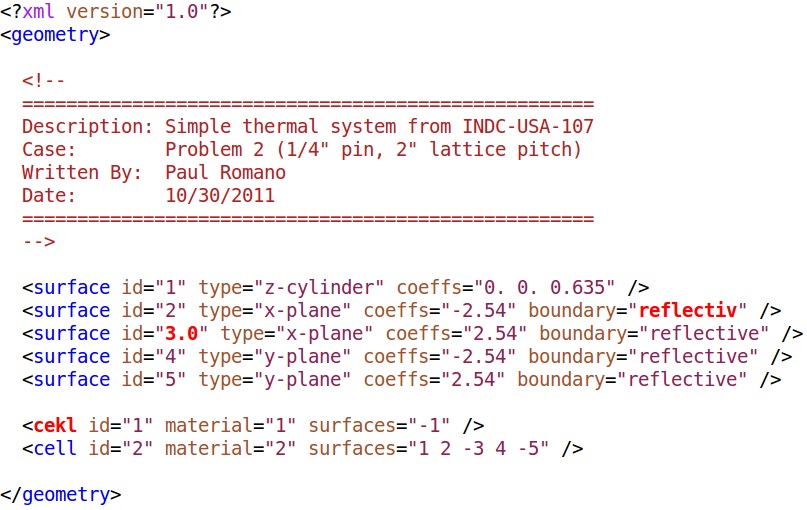
\includegraphics[width=0.5\textwidth]{images/relaxng.png}
  \caption{Example of an XML input file in GNU Emacs being validated against a
    corresponding RELAX NG schema in real-time. Errors in the input are
    automatically highlighted in red.}
  \label{fig:relaxng}
\end{figure}

\subsubsection{Output}

When a simulation in OpenMC completes, a number of output files are written to
disk. The number and format of these files depends on how the code was compiled
and what options are given in the user input. The most common output files
include:
\begin{enumerate}
\item \textbf{tallies.out} -- plain text ASCII file listing the mean and
  standard deviation (or confidence interval half-width) for each tally bin. For
  simple problems with only a few tallies, this file is likely adequate for
  analyzing results.
\item \textbf{State point files} -- binary files containing all the
  information needed either to determine confidence intervals for tallies or to
  restart the run completely. By default, one state point file is written at the
  end of the simulation, but the user can specify particular batches at which
  state points should be written.
\end{enumerate}
In addition to these files, numerous other output files may be generated at the
request of the user or upon hitting an error in the code.

State point files are the primary means of obtaining, interpreting, and
post-processing tally results.  By itself, a state point file is not very useful
since it is in an arbitrary binary format. However, a Python module,
statepoint.py, is available that makes it easy and intuitive to extract and
visualize tally results. In addition, a graphical user interface built on top of
the statepoint.py module and PyQt provides mesh tally
plotting. \autoref{fig:meshplot} shows a screenshot of the PyQt mesh tally
plotting application. Alternatively, a separate Python utility is provided to
process mesh tallies from statepoints into VTK or SILO files.  For example,
\autoref{fig:3dplot} shows a 3D visualization of a mesh tally in ParaView.
\begin{figure}[htb]
  \centering
  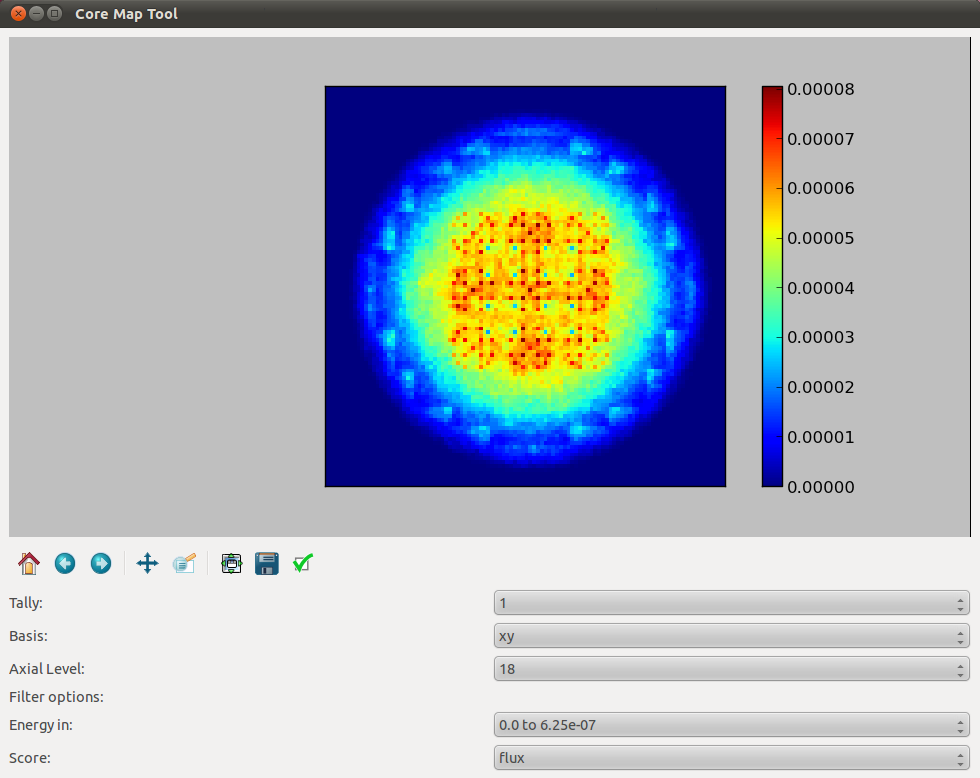
\includegraphics[width=0.5\textwidth]{images/plotmeshtally.png}
  \caption{Example of PyQt mesh tally plotting application displaying a radial
    flux distribution.}
  \label{fig:meshplot}
\end{figure}
\begin{figure}[htb]
  \centering
  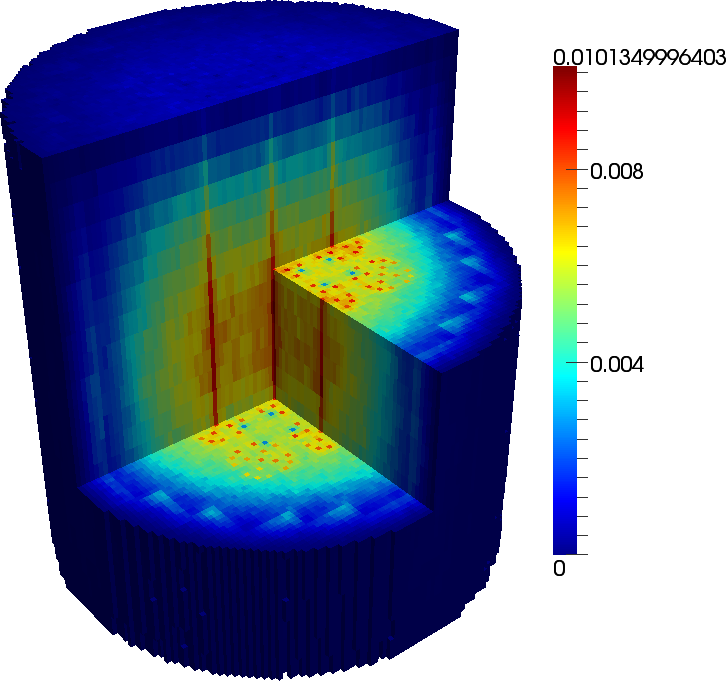
\includegraphics[width=0.4\textwidth]{images/tallyplot.png}
  \caption{Example of a 3D visualization of a mesh tally using ParaView.}
  \label{fig:3dplot}
\end{figure}

State point files (and other binary files) can be written either in a raw binary
format or in HDF5 format. While the HDF5 format should be preferred and ensures
portability across different architectures, the former is made available to
ensure that users can take advantage of state point capabilities even on systems
where HDF5 is unavailable.

One recent capability added to OpenMC is the ability to create \textbf{particle
  restart files}. These files contain a particle's attributes at birth, as well
as the random number seed used to start its history, and are created whenever
OpenMC hits a ``fatal error'' related to geometry tracking causing it to
abort. This allows the particle history to be simulated in order to better
determine what caused OpenMC to abort unexpectedly.

\subsection{Documentation}

Extensive documentation for the OpenMC code is available online at
\url{http://mit-crpg.github.io/openmc}. The documentation consists of the
following major pieces:
\begin{itemize}
\item \textbf{Release notes} describing what changes were made between
  subsequent releases, what new features were introduced, what bugs were fixed,
  and what platforms the code is known to run on.
\item A \textbf{theory and methodology} section describing in detail the
  algorithms used for geometry, cross sections, random number generation,
  physics, tallies, $k$-eigenvalue calculations, and parallelization in OpenMC
  including derivations of key equations. This section contains a wealth of
  information and should be the first stop for anyone wondering how the code
  works.
\item A \textbf{user's guide} that describes how to build and install OpenMC,
  how to write XML input files and the various elements available, how to
  post-process results and visualize data, and a troubleshooting guide.
\item A \textbf{developer's guide} that contains a description of important data
  structures and variables, a style guide for developers active on the master
  branch OpenMC, and binary file format specifications.
\end{itemize}
In addition to the online documentation, users and developers can discuss
various issues on separate Google Groups mailing lists.

All documentation for OpenMC is written in a markup language called
reStructuredText. This markup format can be parsed and translated by Sphinx
\cite{sphinx-2013} to produce documentation as a website (.html), a PDF, or
various other formats.

\subsection{Version Control and Workflow}

All version control of OpenMC and its documentation is handled through the git
distributed revision control system. In addition to git, the web-based hosting
service GitHub is used to provide a central host, issue/milestone tracking,
workflow control via pull requests, a wiki, and documentation hosting. The
combination of git and GitHub enables developers to maintain high productivity
in collaborating with one another, testing out new ideas, and documenting their
work.

Active development on OpenMC is conducted using an integration-manager workflow
as described by Chacon \cite{chacon-2009}. This workflow works particularly well
with the GitHub hosting service that is used by OpenMC. On GitHub, each
developer can easily fork a project creating their own public copy of the OpenMC
repository. They are then free to make whatever changes and modifications they
wish and are not required to have any special access on the original
repository. If a developer wants their changes to be merged into the official
project, they can issue a \emph{pull request} --- at this point, the person
designated as the integration manager then reviews the request and, if the
changes are acceptable, merges it in. \autoref{fig:workflow} illustrates the
general integration-manager workflow.
\begin{figure}[htb]
  \centering
  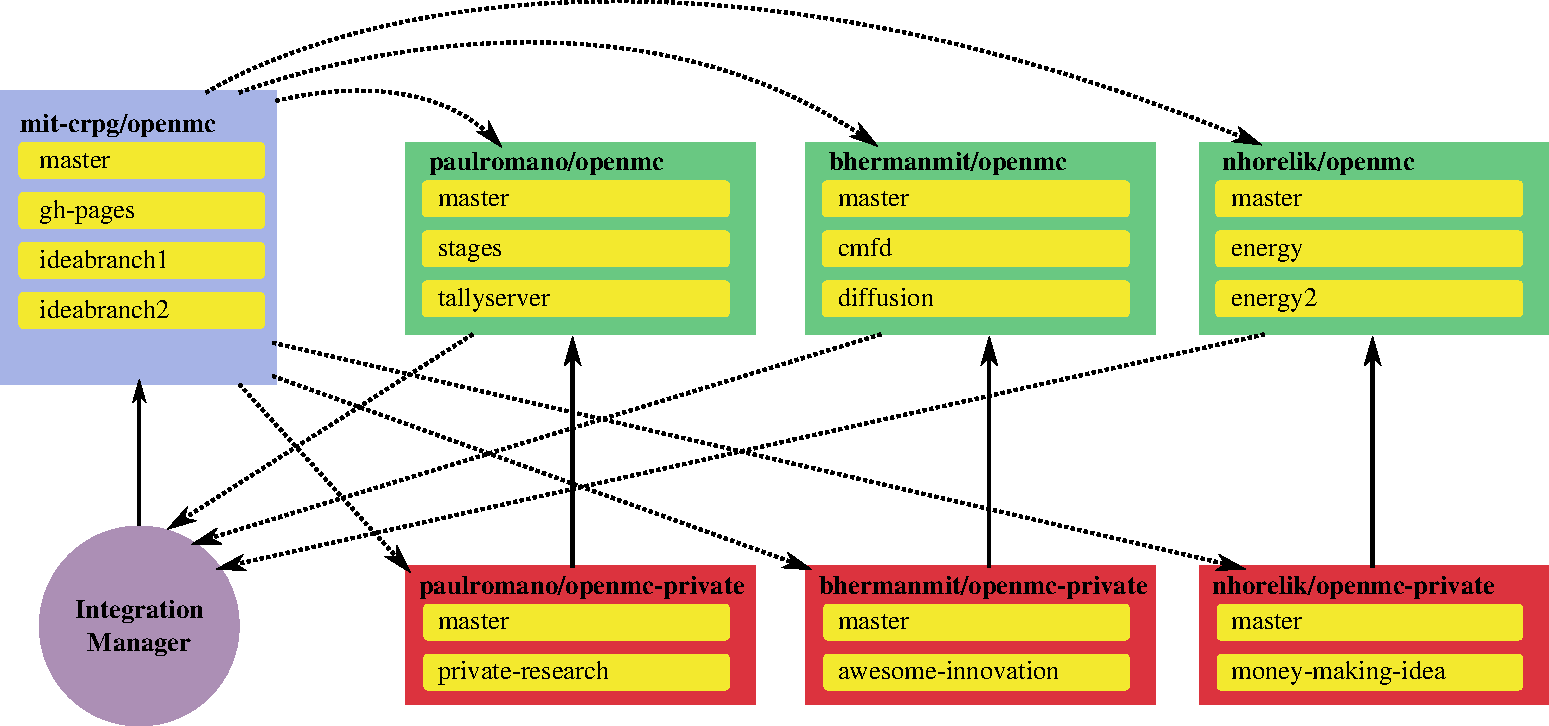
\includegraphics[width=0.5\textwidth]{images/integration-manager.pdf}
  \caption{Integration manager workflow pattern used in OpenMC development.}
  \label{fig:workflow}
\end{figure}

%%%%%%%%%%%%%%%%%%%%%%%%%%%%%%%%%%%%%%%%%%%%%%%%%%%%%%%%%%%%%%%%%%%%%%%%%%%%%%%%
\section{Licensing}

OpenMC is licensed under the MIT/X open source license. This permissive license
allows any user to copy, modify, redistribute, and even sell the software if
they so wish. Unlike copyleft licenses such as the GNU General Public License,
it does not require that modifications to the code be released under the same
license, and thus commercial entities are free to use any part of the code
within their own proprietary software without having to release it for free.

%%%%%%%%%%%%%%%%%%%%%%%%%%%%%%%%%%%%%%%%%%%%%%%%%%%%%%%%%%%%%%%%%%%%%%%%%%%%%%%%
\section{Conclusions}

OpenMC has been developed from scratch with a focus on high-performance
algorithms and modern software development practices. While the code is
relatively young, it is already being used in a number of advanced R\&D projects
including the Consortium for Advanced Simulation of LWRs and the ANL Center for
Exascale Simulation of Advanced Reactors. OpenMC is available as free software
under an open source license, enabling wider collaboration within the nuclear
science and engineering community.

%%%%%%%%%%%%%%%%%%%%%%%%%%%%%%%%%%%%%%%%%%%%%%%%%%%%%%%%%%%%%%%%%%%%%%%%%%%%%%%%
\section*{Acknowledgments}

This research was performed under appointment of the first and third authors to
the Rickover Fellowship Program in Nuclear Engineering sponsored by Naval
Reactors Division of the U.S. Department of Energy. This work was also supported
in part by the Consortium for Advanced Simulation of Light Water Reactors, an
Energy Innovation Hub for Modeling and Simulation of Nuclear Reactors under
U.S. Department of Energy Contract No. DE-AC05-00OR22725, and by the Office of
Advanced Scientific Computing Research, Office of Science, U.S. Department of
Energy, under Contract DE-AC02-06CH11357.

%%%%%%%%%%%%%%%%%%%%%%%%%%%%%%%%%%%%%%%%%%%%%%%%%%%%%%%%%%%%%%%%%%%%%%%%%%%%%%%%
\bibliographystyle{ans}
\bibliography{references}
\end{document}
